Простейшие классические методы перестроения выполняются в предположении, что направление смещения узла совпадает с нормалью, проведенной из этого узла.
Таким образом, необходимо лишь определить величину смещения.
Отметим, что в двумерной постановке можно найти оптимальное решение (обеспечивающее минимальное отклонение по объему от целевого значения) поставленной задачи \cite{Rybakov_2D}.

\begin{figure}[h]
  \centering
  \begin{minipage}[h]{0.49\textwidth}
    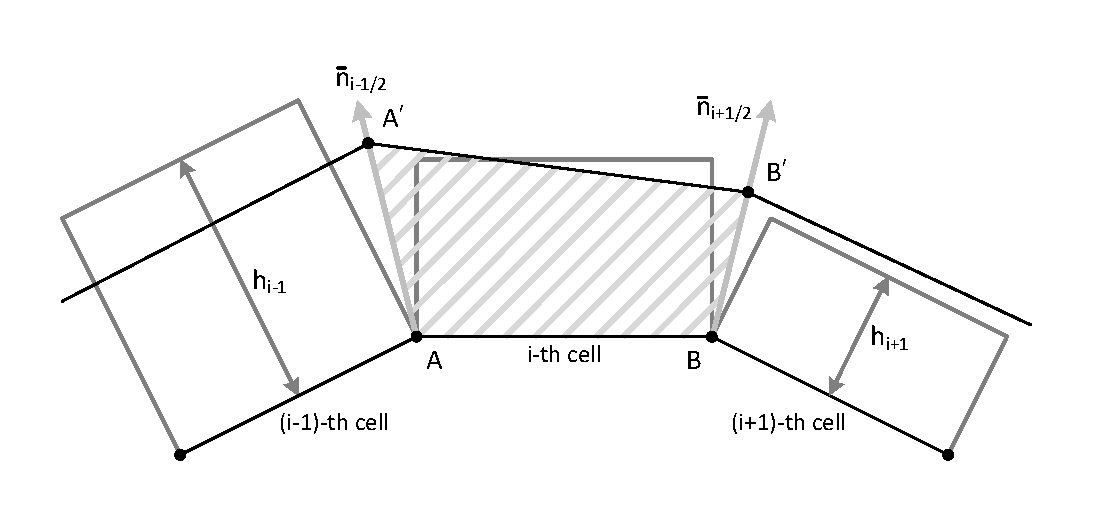
\includegraphics[width=\textwidth]{pics/pic_classical_methods_rectangles_size.pdf}
    \caption{Перестроение поверхности с помощью метода прямоугольников в 2D.}\label{fig:pic_classical_methods_rectangles}
  \end{minipage}
  \hfill
  \begin{minipage}[h]{0.49\textwidth}
    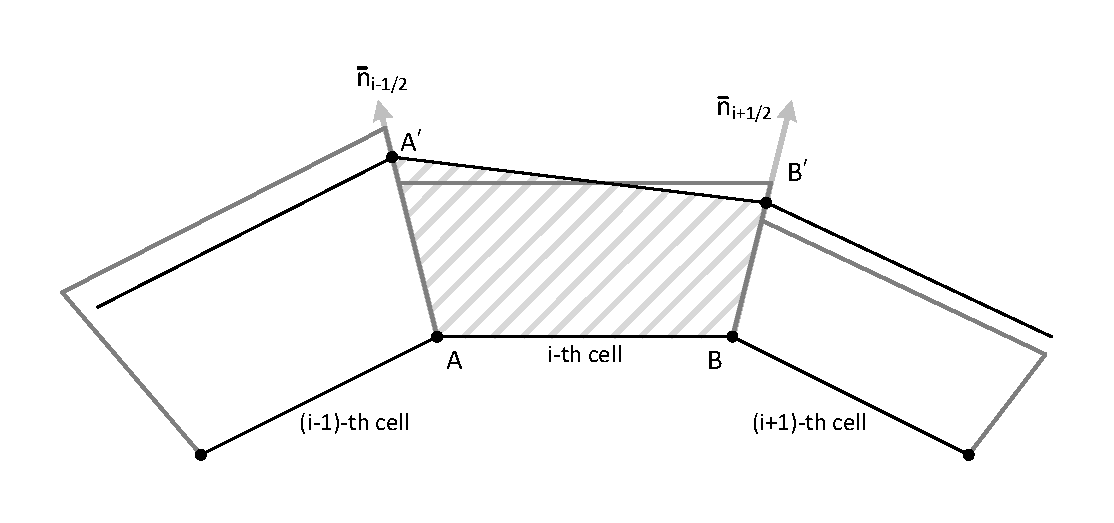
\includegraphics[width=\textwidth]{pics/pic_classical_methods_trapezoids_size.pdf}
    \caption{Перестроение поверхности с помощью метода трапеций в 2D.}\label{fig:pic_classical_methods_trapezoids}
  \end{minipage}
\end{figure}

В качестве первого метода рассмотрим метод призм (в двумерной постановке аналогом данного метода является метод прямоугольников, продемонстрированный на Fig.~\ref{fig:pic_classical_methods_rectangles}).
В этом методе входными данными является объем накопленного льда в каждой ячейке сетки ($V(f)$).
На первым шаге в каждой ячейке ищется толщина ледяного покрова в предположении, что лед в пределах одной ячейки имеет форму призмы, и ячейка является основанием этой призмы.
Тогда толщина ледяного покрова равняется $h(f) = \frac{V(f)}{S(f)}$, где $S(f)$ -- площадь ячейки.
После чего величина смещения каждого узла вычисляется просто как среднее арифметическое высот ледяного покрова во всех инцидентных ячейках:

\begin{equation}
h(N) = \frac{1}{|\mathscr{F}(N)|} \sum_{f \in \mathscr{F}(N)}{h(f)}
\end{equation}

Второй метод можно назвать методом пирамид (в двумерной постановке аналогом данного метод является метод трапеций, показанный на Fig.~\ref{fig:pic_classical_methods_trapezoids}).
Входными данными также является объем накопленного льда в каждой ячейке сетки ($V(f)$).
Однако в отличие от предыдущего метода объем накопленного в ячейке льда представляется не призмой, а усеченной пирамидой, основанием которой является ячейка, а боковые ребра направлены вдоль нормалей узлов.
Высота этой усеченной пирамиды ищется из соотношения $V(f) = \frac{1}{3} h (2S + hS'_h + \sqrt{S(S + hS'_h)})$, где величина $S'_h$ определяется направлениями нормалей узлов ячейки.
Тогда как узлы ячейки являются точками первого основания построенной пирамиды, точки второго основания представляют собой новые положения узлов, вычисленных относительно рассматриваемой ячейки.
Таким образом, у каждого узла сетки вычисляется несколько новых положений (каждое из которых вычислено относительно своей инцидентной ячейки).
Для двумерного случая получается ровно два таких новых положения (так как в двумерном случае каждый узел имеет ровно две инцидентные ячейки), для трехмерного случае таких точек более двух.
Для выбора единственного нового положения узла сетки берется среднее значение из всех положений, вычисленных относительно инцидентных ячеек.

Из рассмотренных двух методов интуитивно создается впечатление, что метод пирамид должен быть более точным, так как он учитывает потери и избыток объема льда, образующиеся из-за изломов сетки (так как соседние ячейки не лежат в одной плоскости, то представление льда в ячейках в виде призм неизбежно приводит к образованию пробелов или наложений частей льда в виде призм друг на друга).
Но по крайней мере в двумерном случае это предположение оказывается неверным, так как метод прямоугольников демонстрирует меньшее отклонение от точного решения по сравнению с методом трапеций \cite{Rybakov_2D}.

\begin{figure}[h]
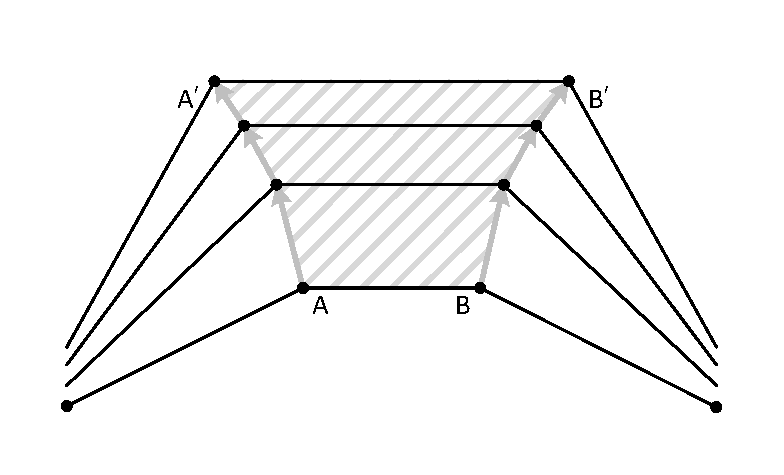
\includegraphics[width=0.48\textwidth]{pics/pic_classical_methods_multilayer_size.pdf}
\captionstyle{center}\caption{Многослойное перестроение сетки.}\label{fig:pic_classical_methods_multilayer}
\end{figure}

Вне зависимости от используемого метода перестроения значительно повысить точность можно с помощью многослойного подхода \cite{BourgaultCote}.
В этом случае вместо однократного перестроения сетки по объему накопленного льда в каждой ячейке ($V(f)$), выбирается фиксированное количество шагов перестроения $k$, а дальше процедура выполняется $k$ раз подряд, но с использованием объема накопленного в ячейке льда $\frac{V(f)}{k}$.
Точность повышается из-за того, что после каждого шага перестроения нормали в узлах сетки меняют свое направление, и общий объем наращиваемого льда становится более криволинейным, лучше учитывает геометрию сетки и, как следствие, точнее соответствует исходному значению $V(f)$ (см. Fig.~\ref{fig:pic_classical_methods_multilayer}).